\documentclass[a4paper]{report}
% define the title
\usepackage{textcomp}
\usepackage{mcode}
\usepackage{amsmath}
\newcommand\numberthis{\addtocounter{equation}{1}\tag{\theequation}}
\usepackage{graphicx}
\graphicspath{ {images/} }
\usepackage{subcaption}
%\usepackage[x11names]{xcolor}                     %Additional colors
\usepackage{tikz}
\usepackage{euler}
\usepackage[hidelinks]{hyperref}
\author{Nandakishore MM}
\title{BTP Project Report}
\begin{document}
	% generates the title
	\maketitle
	
	\newpage
	\tableofcontents
	\newpage
	\listoffigures
	\newpage
	\listoftables
	\newpage
	
	
	\chapter{Introduction}
	In this report we introduce and describe the implementation of multigrid methods, GPU and parallel programming using CUDA and OpenMP and application variational principles for plane compressible flow calculations. 
	
	Multigrid methods in numerical analysis are a group of algorithms for solving differential equations using a hierarchy of discretizations.
	The main idea of multigrid is to accelerate the convergence of a basic iterative method by global correction from time to time, accomplished by solving a similar problem on a coarser grid.
	Multigrid methods are among the fastest solution techniques known today.
	In contrast to other methods, multigrid methods are general in that they can treat arbitrary regions and boundary conditions as they do not depend any special properties of the equation.
	There are many variations of multigrid algorithms, but the common features are that a hierarchy of discretizations (grids) is considered. The important steps are \cite{multigrid}-
	\begin{itemize}
		\item \textbf{Smoothing} – reducing high frequency errors, for example using a few iterations of the Gauss–Seidel method.
		\item \textbf{Restriction} – downsampling the residual error to a coarser grid.
		\item \textbf{Interpolation} or \textbf{prolongation} – interpolating a correction computed on a coarser grid into a finer grid.
	\end{itemize}
	
	\textbf{CUDA}, which stands for Compute Unified Device Architecture, is a parallel computing platform and programming model created by NVIDIA and implemented by the graphics processing units (GPUs) that they produce.
	GPUs are highly parallel multi-core systems allowing very efficient manipulation of large blocks of data. 
	This design is more effective than general-purpose CPUs for algorithms where processing of large blocks of data is done in parallel.
	A typical CFD problem involves solving for the flow variables using an iterative method on a grid. Each update on a grid points involves calculations using a few surrounding grid points. This procedure can be efficiently run in parallel.
	C/C++ programmers use 'CUDA C/C++', compiled with "nvcc", to program or convert existing code to run on the GPU. 
	
	OpenMP is an API for shared memory parallel programming in C/C++ and Fortran. It is ideal for running on multi core CPUs.

	The classical problem of steady inviscid subsonic flow past an aerofoil can be formulated in two ways. 
	The usual formulation is as a boundary value problem consisting of a set non linear partial differential equations and a set of boundary conditions. 
	However, it can also be formulated in terms of complementary variational principles. 
	This method consists of replacing the infinitely dimensional variational problem by a finitely dimensional problem by means of finite differences, and an approximate maximizing function is then found by standard methods. This method is discussed in detail by H. Rasmussen, and N. Heys \cite{rasmussen}
	
	\chapter{Multigrid Methods}
	
	\section{Model Problem}
	Consider a large sparse linear system of equations $A \mathbf{u}=\mathbf{f}$, 
	where $A$ is a $n \times n$ matrix.
	Let us denote $\mathbf{v}$ for the approximate solution obtained using some iterative method.
	
	In later sections the $j$th component of $\mathbf{u}$ and $\mathbf{v}$ will be denoted as $u_j$ and $v_j$.
	When associating $\mathbf{u}$ and $\mathbf{v}$ with a particular grid, say $\Omega^h$ ( where $h$ is the grid spacing ), the notation $\mathbf{u}^h$ and $\mathbf{v}^h$ are used.
	
	As an example the following model problem is considered in the following sections -
	\begin{equation}
	\label{model}
	-u''(x) = f(x), \qquad 0<x<1
	\end{equation}
	\begin{equation}
	u(0) = u(1) = 0
	\end{equation}
	This problem can be discretized as follows
	\begin{equation}
	-u_{j-1} + 2u_j - u_{j+1} = h^2 f_j, \qquad 1 \leq j \leq n-1
	\end{equation}
	\begin{equation}
	u_0 = u_n = 0
	\end{equation}
	
	\section{Residual and error}
	
	Define the algebraic error as $$ \mathbf{e} = \mathbf{u} - \mathbf{v} $$
	The error is a vector and it magnitude can be measured by any of the standard vector norms.
	The Euclidean or 2-norm is defined by 
	$$ || \mathbf{e} ||_2 = 	\left\lbrace \sum_{j=1}^n e^2_j \right\rbrace^{1/2} $$
	A computable measure of how well $\mathbf{v}$ approximated $\mathbf{u}$ is given by the residual
	$$ \mathbf{r} = \mathbf{f} - A\mathbf{u} $$
	
	\section{Basic Iterative Methods} \label{iter}
	
	\subsection{Jacobi Iteration}
	The Jacobi iteration in component for can be expressed as
	\begin{equation}
	v_j^{(1)} = \frac{1}{2}\left( v_{j-1}^{(0)} + v_{j+1}^{(0)} + h^2 f_j \right), \qquad 1 \leq j \leq n-1.
	\end{equation}
	where $v^{(0)}$ denotes the current approximation and $v^{(1)}$ denotes the new and updated approximation

	\subsection{Weighted Jacobi Iteration}
	The first step in weighted Jacobi iteration is to compute
	$$
	v_j^{*} = \frac{1}{2}\left( v_{j-1}^{(0)} + v_{j+1}^{(0)} + h^2 f_j \right), \qquad 1 \leq j \leq n-1.
	$$
	Then, the new approximation is given by
	\begin{equation}
	v_j^{(1)} = (1-\omega) v_{j}^{(0)} + \omega v_{j}^{*}, \qquad 1 \leq j \leq n-1.
	\end{equation}
	
	\subsection{Gauss-Seidel Iteration}
	The Gauss-Seidel iteration is similar to Jacobi iteration except that the components of the new iteration are used as soon as they are computed.
	This can be expressed as 
	\begin{equation}
	v_j \longleftarrow \frac{1}{2}\left( v_{j-1} + v_{j+1} + h^2 f_j \right), \qquad 1 \leq j \leq n-1.
	\end{equation}
	where $\longleftarrow$ stands for replacement or overwriting
	
	\subsection{Red-Black Gauss-Seidel Iteration}
	This is the same as Gauss-Seidel method except that all even components are updated first by the expression
	\begin{equation}
	v_{2j} \longleftarrow \frac{1}{2}\left( v_{2j-1} + v_{2j+1} + h^2 f_{2j} \right)
	\end{equation}
	and then all odd components using
	\begin{equation}
	v_{2j+1} \longleftarrow \frac{1}{2}\left( v_{2j} + v_{2j+2} + h^2 f_{2j+1} \right)
	\end{equation}
	The advantage of red-black over regular Gauss-Seidel is in terms of parallel processing.
	The red points need only the black points for updating and therefore be updated in any order. This can be done by several independent processors. The same is applicable for the black points.
	
	\subsection{Drawbacks of the basic iterative methods}
	Let us assume the initial guess to the above model problem consists of the following Fourier modes
	$$
	v_j = \sin \left( \frac{jk\pi}{n} \right), \qquad 0 \leq j \leq n,
	\qquad 1 \leq k \leq n-1
	$$
	where $k$ represents the wave number.
	The modes in the lower half of the spectrum  with wavenumbers in the range $1 \leq k < n/2 $, are called \textit{law frequency} or \textit{smooth modes}. The modes in the upper half of the spectrum , with $n/2 \leq k \leq n-1$ are called \textit{high-frequency} or \textit{oscillatory modes}.
	An analysis of the weighted Jacobi iteration will give the following expression for the convergence of various modes
	$$\lambda_k = 1-2\omega\sin^2 \left(\frac{k\pi}{2n}\right)$$
	Convergence is better when $|\lambda_k|$ is small.
	\begin{figure}[hbtp]
	\centering
	\includegraphics[scale=.5]{convergence_weighted_jacobi.png}
	\caption{$\lambda_k$ vs wave number $k$ for different $\omega$ for weighted Jacobi iterations}\label{conv_wj}
	\end{figure}
	From figure \ref{conv_wj} \cite{multigrid}, it can be seen that while the high frequency modes have a nominal damping rate, the smooth mode damp very slowly. Many relaxation schemes possess\ this property of eliminating the oscillatory modes and leaving the smooth modes. This is called \textit{smoothing property} and is a serious limitation of conventional relaxation methods.
	However this limitation can be overcome using multigrid methods. 
	
	
	\section{Basic Multigrid methods}
	One of the ways to improve a relaxation scheme is to use a good initial guess. A well-known technique is to perform some preliminary iterations on a coarser grid which is inexpensive. 
	Another important property of a coarser grid is how the various Fourier modes on the finer grid are represented on it. 
	Consider the kth mode  on the fine grid $\Omega^h$ evaluated at the even numbered grid points ( Note: The grid points of the coarse grid $\Omega^{2h}$ are the even no. grid points on the fine grid $\Omega^h$ ). If $1\leq k<n/2$. its components can be written as
	$$
	w^h_{k,2j} = \sin \left( \frac{2jk\pi}{n} \right) =
	\sin \left( \frac{jk\pi}{n/2} \right) = w^{2h}_{k,j}
	$$
	We see that the smooth components on $\Omega^h$ is more oscillatory on the coarse grid $\Omega^{2h}$. This can be useful in overcoming the smoothing property of the relaxation schemes.
	
	\subsection{Residual equation}
	If $\mathbf{v}$ is the approximation to the exact solution $\mathbf{u}$, then the error is given by
	$$ \mathbf{e} = \mathbf{u} - \mathbf{v}$$ 
	Then
	$$ A\mathbf{e} = A\mathbf{u} - A\mathbf{v}$$
	$$ A\mathbf{e} = \mathbf{f} - A\mathbf{v}$$
	\begin{equation}
	A\mathbf{e} = \mathbf{r}
	\end{equation}
	The last equation above is called the \textit{residual equation}. It can be interpreted as follows
	
	Relaxation of the original equation $A\mathbf{u}=\mathbf{f}$ with an arbitrary initial guess $\mathbf{v}$ is equivalent to relaxing on the residual equation $A\mathbf{e} = \mathbf{r}$ with the specific initial guess $\mathbf{e} = 0$ 
	
	\subsection{Intergrid transfer operators}
	The process of transferring approximation from the coarser grid to the finer grid is called \textit{interpolation} or \textit{prolongation}. The linear interpolation operator, denoted by $I_{2h}^h$ takes the coarse-grid vectors and produces the fine grid vectors according to the rule $I_{2h}^h v^{2h} = v^h$; is given by
	\begin{align*}
	v_{2j}^h &= v_j^{2h},\\
	v_{2j+1}^h &= \frac{1}{2}\left( v^{2h}_j + v^{2h}_{j+1} \right),
	\qquad 0 \leq j \leq \frac{n}{2} - 1
	\end{align*}
	For 2 dimensional problems $I_{2h}^h$ is given by
	\begin{align*}
	v_{2i,2j}^h &= v_{i,j}^{2h},\\
	v_{2i+1,2j}^h &= \frac{1}{2}\left( v^{2h}_{i,j} + v^{2h}_{i+1,j} \right), \\
	v_{2i,2j+1}^h &= \frac{1}{2}\left( v^{2h}_{i,j} + v^{2h}_{i,j+1} \right), \\
	v_{2i+1,2j+1}^h &= \frac{1}{4}\left( v^{2h}_{i,j} + v^{2h}_{i+1,j} + v^{2h}_{i,j+1} + v^{2h}_{i+1,j+1} \right), \\
	\qquad 0 \leq 1&,j \leq \frac{n}{2} - 1
	\end{align*}
	
	The other intergrid transfer operator is the restriction operator denoted by $I^{2h}_h$. It moves vectors from the fine grid to a coarse grid. It is given by the full weighted restriction operator
	\begin{equation}
	v^{2h}_j = \frac{1}{4} \left( v^h_{2j-1} + v^h_{2j} + v^h_{2j+1} \right), \qquad 0 \leq j \leq \frac{n}{2} - 1
	\end{equation}
	In 2 dimension the same is given by
	\begin{align*}
	v^{2h}_{ij} = \frac{1}{16}[
	v^h_{2i-1,2j-1} &+ v^h_{2i+1,2j-1} + v^h_{2i-1,2j+1} + v^h_{2i+1,2j+1} \\
	&+ 2 (v^h_{2i,2j-1} + v^h_{2i,2j+1} + v^h_{2i-1,2j} + v^h_{2i+1,2j} )  \\
	&+ v^h_{2i,2j}
	], \qquad 1 \leq i,j \leq \frac{n}{2}-1
	\end{align*}
	
	\subsection{Two grid Correction Scheme}
	The two grid correction scheme can be defined by the following algorithm.
	$$ \mathbf{v}^h \leftarrow \text{TG}(\mathbf{v}^h, \mathbf{f}^h) $$
	\begin{itemize}
	\item Relax $\nu_1$ times  on $A^h\mathbf{u}^h = \mathbf{f}^h$ on $\Omega^h$ with initial guess $\mathbf{v}$
	\item Compute the fine-grid residual  $\mathbf{r}^h = \mathbf{f}^h - A\mathbf{v}^h$ and restrict it to the coarse grid by $\mathbf{r}^{2h} = I_h^{2h} \mathbf{r}^h$.
	\item Solve $A^{2h} \mathbf{e}^{2h} = \mathbf{r}^{2h}$ on $\Omega^{2h}$
	\item Interpolate the coarse-grid error to the fine grid by $\mathbf{e}^h=I^h_{2h}\mathbf{e}^{2h}$ and correct the fine grid approximation by $\mathbf{v}^h \leftarrow \mathbf{v}^h + \mathbf{e}^h$
	\item Relax $\nu_2$ times  on $A^h\mathbf{u}^h=\mathbf{f}^h$ with initial guess $\mathbf{v}$
	\end{itemize}
	
	\subsection{Multigrid Scheme ( V Cycle )}
	
	In the two grid  correction scheme, the coarse grid problem can be solved using the two grid correction scheme itself. This can be recursively applied to successive coarse grid problems. This is the basis for \textit{V cycle scheme}. 
	
	To simplify notations,  let us call the right side of the  residual equation $\mathbf{f}^{2h}$, rather than $\mathbf{r}^{2h}$, the solution of the residual equation $\mathbf{e}^{2h}$ as $\mathbf{u}^{2h}$, and $\mathbf{v}^{2h}$ denotes the approximation to the solution $\mathbf{u}^{2h}$.
	
	Now the V cycle scheme can be defined as follows
	\subsubsection{V Cycle Scheme}
	$$ \mathbf{v}^h \leftarrow V^h(\mathbf{v}^h, \mathbf{f}^h) $$
	\begin{enumerate}
	\item Relax $\nu_1$ times on $A^h\mathbf{u}^h = \mathbf{f}^h$ with a given initial guess $\mathbf{v}^h$.
	\item If $\Omega^h = $ coarsest grid, then go to step \textbf{4}. \\
	Else
	\begin{align*}
	\mathbf{f}^{2h} &\leftarrow I_h^{2h}(\mathbf{f}^{h} - A^h\mathbf{v}^{h}), \\
	\mathbf{v}^{2h} &\leftarrow 0, \\
	\mathbf{v}^{2h} &\leftarrow V^{2h}(\mathbf{v}^{2h}, \mathbf{f}^{2h}).
	\end{align*}
	\item Correct $\mathbf{v}^h \leftarrow \mathbf{v}^h + I_{2h}^h\mathbf{v}^{2h}$.
	\item Relax $\nu_2$ times  on $A^h \mathbf{u}^h = \mathbf{f}$ with initial guess $\mathbf{v}^{h}$
	\end{enumerate}
	
	\subsection{$\mu$ Cycle}	
	Now the $\mu$ cycle scheme can be defined as follows
	\subsubsection{$\mu$ Cycle Scheme}
	$$ \mathbf{v}^h \leftarrow \mu^h(\mathbf{v}^h, \mathbf{f}^h) $$
	\begin{enumerate}
	\item Relax $\nu_1$ times on $A^h\mathbf{u}^h = \mathbf{f}^h$ with a given initial guess $\mathbf{v}^h$.
	\item If $\Omega^h = $ coarsest grid, then go to step \textbf{4}. \\
	Else
	\begin{align*}
	\mathbf{f}^{2h} &\leftarrow I_h^{2h}(\mathbf{f}^{h} - A^h\mathbf{v}^{h}), \\
	\mathbf{v}^{2h} &\leftarrow 0, \\
	\mathbf{v}^{2h} &\leftarrow \mu^{2h}(\mathbf{v}^{2h}, \mathbf{f}^{2h}) \text{ $\mu$ times }.
	\end{align*}
	\item Correct $\mathbf{v}^h \leftarrow \mathbf{v}^h + I_{2h}^h\mathbf{v}^{2h}$.
	\item Relax $\nu_2$ times  on $A^h \mathbf{u}^h = \mathbf{f}$ with initial guess $\mathbf{v}^{h}$
	\end{enumerate}
	When $\mu=1$, it degenerates to V cycle scheme. $\mu=2$ is called W cycle.
	
	\subsection{Full Multigrid (FMG)}
	The above methods can be optimised more by providing a good initial guess on every grid. This is done using the Full Multigrid (FMG) V cycle
	
	\subsubsection{Full Multigrid V-Cycle}
	$$ \mathbf{v}^h \leftarrow \text{FMG}^h(\mathbf{f}^h) $$
	\begin{enumerate}
	\item If $\Omega^h = $ coarsest grid, set $\mathbf{v}^h = 0$, go to step \textbf{3}. \\
	Else
	\begin{align*}
	\mathbf{f}^{2h} &\leftarrow I_h^{2h}(\mathbf{f}^{h}), \\
	\mathbf{v}^{2h} &\leftarrow \text{FMG}^{2h}(\mathbf{f}^{2h}) \text{ $\mu$ times }.
	\end{align*}
	\item Correct $\mathbf{v}^h \leftarrow I_{2h}^h\mathbf{v}^{2h}$.
	\item $\mathbf{v}^{h} \leftarrow V^h(\mathbf{v}^h, \mathbf{f}^h)$ $\nu_0$ times
	\end{enumerate}
	
	\section{Application}
	
	\subsection{Problem}
	The multigrid algorithms discussed above is applied to the following problem-
	\begin{equation}
	\frac{\partial^2 u}{\partial x^2} + \frac{\partial^2 u}{\partial x^2} = 0
	\end{equation}
	subject to boundary conditions
	\begin{align}
	u(x,0) &= x^2, \\
	u(0,y) &= y^2, \\
	u(x,1) &= 1-x^2, \\
	u(1,y) &= 1-y^2.
	\end{align}
	
	\subsection{Results}
	\subsubsection{Solution}
	For obtaining solution a Red Black Gauss Seidel iteration has been used. The solver was run on a grid of size $4097 \times 4097$ (16 million grid points). The solution is plotted in figures \ref{sol1} and \ref{sol2}
	
	\begin{figure}[hbtp]
	\centering
	\includegraphics[scale=.8]{mg_solution_1.png}
	\caption{Solution of the boundary value problem on a $4097 \times 4097$ grid} \label{sol1}
	\end{figure}
	
	\begin{figure}[hbtp]
	\centering
	\includegraphics[scale=.8]{mg_solution_2.png}
	\caption{Solution of the boundary value problem on a $4097 \times 4097$ grid} \label{sol2}
	\end{figure}
	
	\subsubsection{Comparison of multigrid schemes}
	For comparing different multigrid schemes, let us define a work unit (WU) as the one iteration on the finest grid.
	Hence one iteration on the next coarsest grid is equivalent to 1/4 WU and so on.
	
	The comparisons are presented in figures \ref{v_cycle_comparison} and \ref{mg_comparison}.
	
	\begin{figure}[hbtp]
	\centering
	\includegraphics[scale=.7]{mg_comarison_all_partial.png}
	\caption{Convergence plot different multigrid schemes ( In V($\nu_1$, $\nu_2$), W($\nu_1$, $\nu_2$), FMG($\nu_0$, $\nu_1$, $\nu_2$), $\nu_0$, $\nu_1$ and $\nu_2$ represents the same quantities defined in the algorithm)} \label{mg_comparison}
	\end{figure}

	\begin{figure}[hbtp]
	\centering
	\includegraphics[scale=.7]{mg_v_cycles.png}
	\caption{Convergence plot of V-cycle scheme for different no. of pre relaxation ($\nu_1$) and post relaxation ($\nu_2$) sweeps (V($\nu_1$, $\nu_2$))} \label{v_cycle_comparison}
	\end{figure}	
	
	\newpage	
	
	\begin{table}
	\caption {Time elapsed for convergence for different grid sizes for V-Cycle scheme} \label{scaling_v_cycle_table} 
	\begin{center}
	\begin{tabular}{ c c c c }
	\hline 
	Grid Size & No. of grid points & Time (s) & Ratio\\ 
	\hline 
	257 $\times$ 257 & 66,049 & 0.03 & -\\ 
	513 $\times$ 513 & 263,169 & 0.11 & 3.67\\
	1025 $\times$ 1025 & 1,050,625 & 0.48 & 4.36\\
	2049 $\times$ 2049 & 4,198,401 & 2.07	& 4.31 \\
	4097 $\times$ 4097 & 16,785,409 & 8.43 & 4.07\\ 
	8193 $\times$ 8193 & 67,125,249 & 33.8 & 4.01 \\ 
	\hline 
	\end{tabular} 
	\end{center}
	\end{table}
	
	
	\begin{table}
	\caption {Time elapsed for convergence for different grid sizes for FMG V-Cycle} \label{scaling_fmg_table} 
	\begin{center}
	\begin{tabular}{ c c c c }
	\hline 
	Grid Size & No. of grid points & Time (s) & Ratio\\ 
	\hline 
	257 $\times$ 257 & 66,049 & 0.03 & -\\ 
	513 $\times$ 513 & 263,169 & 0.16 & 5.33\\ 
	1025 $\times$ 1025 & 1,050,625 & 0.79 & 4.94\\ 
	2049 $\times$ 2049 & 4,198,401 & 3.67 & 4.65\\ 
	4097 $\times$ 4097 & 16,785,409 & 6.33 & 4.45\\
	8193 $\times$ 8193 & 67,125,249 & 69.78 & 4.27 \\ 
	\hline 
	\end{tabular} 
	\end{center}
	\end{table}
	
	
	
	\begin{table}
	\caption {Time elapsed for convergence for different grid sizes for iteration without using multigrid} \label{scaling_table} 
	\begin{center}
	\begin{tabular}{ c c c c }
	\hline 
	Grid Size & No. of grid points & Time (s) & Ratio\\ 
	\hline 
	33 $\times$ 33 & 1,089 & 0.02 & -\\ 
	65 $\times$ 65 & 4,225 & 0.34 & 17\\ 
	129 $\times$ 129 & 16,641 & 5.43 & 15.97\\ 
	257 $\times$ 257 & 66,049 & 90.93 & 16.75\\
	\hline 
	\end{tabular} 
	\end{center}
	\end{table}
	
	\subsection{Inference}
	\begin{itemize}
	\item From figure \ref{mg_comparison}, it is clear that multigrid methods perform better than conventional iteration.
	\item The Full Multigrid V-cycle was the fastest algorithm to produce the solution.
	\item Iterations without using any multigrid methods shows a time complexity of $O(n^2)$, as seen from table \ref{scaling_table}. As the no. of grid points become 4 times, the time taken increases to approximately 16 times.
	\item The time elapsed for FMG scheme is found to vary linearly with grid size as seen in table \ref{scaling_fmg_table}. Hence it has a time complexity close to $O(n)$
	\item The time elapsed for V-cycle scheme is found to scale in between the above two schemes (Ref table \ref{scaling_v_cycle_table}). This is in close match with the theoretical prediction of $O(n \log n)$ \cite{multigrid}
	\end{itemize}
	
	\subsection{Conclusion}
	Various multigrid algorithms were explored in this section and there performances were computed. The solver was tested on Laplace equation on a unit square and was run on 67 million grid points.
	
	
	\chapter{Parallel Programming with OpenMP and CUDA}

	\section{Introduction}
		This section discusses about application of parallel programming in numerical simulations. The report is on shared memory architecture of parallel programming using OpenMP and CUDA C/C++. OpenMP is an API for shared memory parallel programming in C/C++ and Fortran. It is ideal for running on multi core CPUs. CUDA is a parallel computing model developed by Nvidia and is implemented by the graphics processing unit(GPU) the produce.	The GPU is a special-purpose CPU, designed with over 100+ processors so that a single instruction works over a large block of data (SIMD/Single Instruction Multiple Data), all of them applying the same operation. 
	
	\section{Basics of Parallel Programming}
	\subsection{Data Parallelism}
	Data Parallelism refers to mode of parallelism where the data is distributed across many processors and all the processors execute the same set of instructions on the data. In the iterative methods discussed in section \ref{iter}, the same calculation is carried out on each grid point independently. Hence this can be easily parallelised.		
	
	\subsection{Data Race}	
	A \textit{data race} is said to occur when two or more threads access the same memory location at the same time with atleast one thread using it for writing. This may lead to ambiguous results and hence should be avoided. This can happen if the wrong algorithm has been chosen to do the parallelism. Taking the case of the iterative methods discussed in section \ref{iter}, the Gauss Seidel iteration will lead a data race conditions. Whereas the Jacobi and Red Black Gauss Seidel methods are suited for parallel computing.

	\subsection{Reduction}
	Reduction refers to given a associative binary operator $\odot$ and an ordered array $s=[a_1 a_2 \dots a_n]$, reduce ($\odot$, $s$) returns $a_1 \odot a_2 \odot \dots \odot a_n$. This is commonly used when taking sum or finding maximum of residuals at every grid point. The common procedure of summing one-by-one takes $O(n)$ operations. But with parallel processors reduction can be done using map reduction algorithm which takes only $O(n \log(n)$ operations and each operation can be performed independently.	
	
	\section{OpenMP}
	OpenMP is fairly easy to implement. It comes along with standard gcc compiler suite. It can be invoked using \textit{-fopenmp} flag during compiling. Some important aspects of OpenMP are discussed below.
	
	\subsection{Parallelising for loops}
	In OpenMP parallelising a for loop involves using the following directive before a for loop.
	\begin{lstlisting}
	# pragma omp parallel for
	\end{lstlisting}
	for example
	\begin{lstlisting}
	# pragma omp parallel for
	for( int i = 0; i < 1000; ++i )
	{
		...
	}
	\end{lstlisting}
	It splits the for loop counter into sections and  distributed it across the processors (threads) to work on independently.
	
	\subsection{Reduction}
	This is implemented in OpenMP using the \emph{reduction} clause. For example, to find the sum of an array
	\begin{lstlisting}
	# pragma omp parallel for reduction(+:sum)
	for( int i = 0; i < 1000; ++i )
	{
		sum += array[i];
	}
	\end{lstlisting}
	and to find the maximum of an array
	\begin{lstlisting}
	# pragma omp parallel for reduction(max:m)
	for( int i = 0; i < 1000; ++i )
	{
		m = max(m, array[i]);
	}
	\end{lstlisting}
	
	\section{CUDA}	
	\subsection{Programming Model}
	A typical program has the following two parts-
	\subsubsection{Kernel or Device Code}
	A kernel is a function callable from the host and executed on the CUDA device simultaneously by many threads in parallel.
	\subsubsection{Host Code}
	The host code is the code run on the CPU. The typical routine of a host code is as follows
	\begin{enumerate}
	\item Initialise the device (GPU)
	\item Allocate memory on GPU
	\item Copy data from the host memory to GPU memory
	\item Execute the kernel code on GPU
	\item Copy the processed data from GPU memory to host memory
	\item Free memory on GPU
	\end{enumerate}
	
	\subsection{Implementing data parallel tasks}
	Here is sample kernel for performing Jacobi iterations
	\begin{lstlisting}
__global__ void Jacobi( float* input,  float* output, 
	unsigned int Ni, unsigned int Nj, float h)
{
	unsigned int i = threadIdx.x + blockIdx.x * blockDim.x; // Y - ID
	unsigned int j = threadIdx.y + blockIdx.y * blockDim.y; // X - ID

	unsigned int iPrev = (i-1)  * Nj + j; // Previous Y element
	unsigned int iNext = (i+1)  * Nj + j; // Next Y element

	unsigned int jPrev = i * Nj + j-1; //Previous X element
	unsigned int jNext = i * Nj + j+1; // Next X element
	
	unsigned int index = i * Nj + j; // Current element

	if( i > 0 && j > 0 && i < (Ni-1) && j <(Nj-1))
		output[index] = 0.25f * (input[iPrev] + input[iNext] 
		+ input[jPrev] + input[jNext] - 4*h*h);
}
	\end{lstlisting}
	The parts of the code is explained below
	
	Keyword \emph{\_\_global\_\_} declares the function as a kernel to be called from the host and executed on the GPU
	\begin{lstlisting}
__global__ void Jacobi( float* input,  float* output, 
	unsigned int Ni, unsigned int Nj, float h)
	\end{lstlisting}
	Each kernel get access to the variables \emph{threadIdx}, \emph{blockIdx} and \emph{blockDim}. The below code calculated \textit{i} and \textit{j} indices from these variables.
	\begin{lstlisting}
{
	unsigned int i = threadIdx.x + blockIdx.x * blockDim.x; // Y - ID
	unsigned int j = threadIdx.y + blockIdx.y * blockDim.y; // X - ID
	\end{lstlisting}
	The kernel code can access only one dimensional array. Hence \textit{i} and \textit{j} has to converted to its 1D equivalent as given below
	\begin{lstlisting}

	unsigned int iPrev = (i-1)  * Nj + j; // Previous Y element
	unsigned int iNext = (i+1)  * Nj + j; // Next Y element

	unsigned int jPrev = i * Nj + j-1; //Previous X element
	unsigned int jNext = i * Nj + j+1; // Next X element

	unsigned int index = i * Nj + j; // Current element
	\end{lstlisting}
	Check boundary  nodes
	\begin{lstlisting}
	if( i > 0 && j > 0 && i < (Ni-1) && j <(Nj-1))
	\end{lstlisting}
	Perform the Jacobi iteration
	\begin{lstlisting}
		output[index] = 0.25f * (input[iPrev] + input[iNext] 
		+ input[jPrev] + input[jNext] - 4*h*h);
}
	\end{lstlisting}
	
	This code is called from the host as follows.
	\begin{lstlisting}
		Jacobi<<<dimGrid,dimBlock>>>(in, out, Ni, Nj, h);
	\end{lstlisting}
	
	\subsection{Reduction}
	Reduction in CUDA can be done using routines in 'Thrust' library that come with the \textit{cuda-toolkit}.
	
	\section{Results}
	The multigrid algorithms implemented in the previous section was modified with CUDA to run on the GPU. The GPU used was Nvidia GeForce GT 630M. The code was also extended to use OpenMP and was tested on a multicore CPU (Intel(R) Core(TM) i5-3317U CPU @ 1.70GHz, 2 cores)
	
	\subsection{Benchmarks}
	
	\begin{table}
	\caption {Time elapsed (in \emph{s}) for convergence for different grid sizes for FMG V-Cycle with CUDA and OpenMP implemented} \label{omp_cuda_table} 
	\begin{center}
	\begin{tabular}{c c c c c c}
	\hline 
	Grid Size & Grid points & Serial Code & OpenMP (1 core) & OpenMP (2 cres) & CUDA \\ 
	\hline 
	65 $\times$ 65 & 4225 & 0.085 & 0.095 & 0.075 & 0.079 \\ 
	129 $\times$ 129 & 16,641 & 1.255 & 1.301 & 0.744 & 0.703 \\ 
	257 $\times$ 257 & 66,049 & 6.261 & 6.282 & 3.489 & 4.492 \\ 
	513 $\times$ 513 & 263,169 & 36.558 & 36.688 & 28.377 & 26.355 \\
	\hline 
	\end{tabular} 
	\end{center}
	\end{table}
	
	\subsection{Conclusion and Remarks}
	\begin{itemize}
	\item OpenMP and CUDA has increased computation performance significantly.
	\item OpenMP code ran 1.29$\times$ faster on 2 cores.
	\item CUDA code ran 1.39$\times$ faster.
	\end{itemize}
	
	
	
			
	
	\chapter{Application of Variational Principles for Plane Compressible flow Calculations}
	
	\section{Introduction}
	The classical problem of steady inviscid subsonic flow past an aerofoil can be formulated in two ways. The usual formulation is as a boundary value problem consisting of a set non linear partial differential equations and a set of boundary conditions. However, it can also be formulated in terms of complementary variational principles. This report describes a variational method for obtaining numerical solutions. The method consists of replacing the infinitely dimensional variational problem by a finitely dimensional problem by means of finite differences, and an approximate maximizing function is then found by standard methods. 

	\section{Formulation}
	
	
	\begin{figure}
		\centering
  		\begin{tikzpicture}
			\draw[thick,<->] (-4.5,0) -- (4.5,0) node[anchor=north west] {x};
			\draw[thick,<->] (0,-4.5) -- (0,4.5) node[anchor=south east] {y};
			\draw[very thick] (0,0) circle(3);
			\draw (2.5,2.5) node {$C$};
			\foreach \y in {-4,-2,...,4}
				\draw[thick, ->] (-7,\y) -- (-5,\y);
			\draw (-6,4.2) node {$U$};
  		\end{tikzpicture}
  		\caption{Sketch of the flow field}
  	\end{figure}	
  	
	The boundary value problem for plane subsonic flow	 past an aerofoil can be formulated as follows.
	
	Let $\vec{u}=(u_1,u_2)$ be the velocity vector in the Cartesian coordinate system. Far from the aerofoil, C $\vec{u}=(U,0)$ where $U$ is a constant.
	
	For an irrotational flow, a velocity potential can be defined as 
	$$ \vec{u} = \nabla \phi$$
	
	The pressure and density are defined by $p$ and $\rho$ respectively. The speed of sound is defined by
	$$c^2=\frac{dp}{d\rho}$$
	
	$$p=p_0 \Biggl(
	1-\frac{q^2}{2\beta c^2_0}
	\Biggr)^\alpha$$

	$$\rho=\rho_0 \Biggl(
	1-\frac{q^2}{2\beta c^2_0}
	\Biggr)^\beta$$	
	
	where
	
	$$q^2 = \vec{u}.\vec{u}, \qquad \alpha=\frac{\gamma}{\gamma-1},
	\qquad \beta=\frac{1}{\gamma-1}$$
	
	the suffix $0$ indicates stagnation values.
	
	The boundary value problem for $\phi$ is equivalent to a variational problem of maximizing the integral 
	\begin{equation} \label{var_eq}
		 J[\phi] = \int_{R_1} pdV + \int_B\phi h dA
	\end{equation}
	($dV = $ area element, $dA = $ arc length element of $B=C$). Then $J[\phi]$ is a maximum if $\nabla.(\rho \vec{u} = 0$ and
	$\rho\vec{u}.\hat{n} = h$ on $B$. Here the normal mass flu $h$ is prescribes on $B$ such that 
	$$ \text{outflow} = \int_B hdA = 0$$
	
	If the flow region $R_1$ becomes infinite, the variational integral (\ref{var_eq}) becomes unbounded. To remove this difficulty, the integral can be formulated as follows
	\begin{equation} \label{var_eq2}
		J[\phi] = \int\int_\infty [ p-p_\infty+p_\infty.\nabla(\phi-\phi_\infty) ]dxdy
	\end{equation}
	
	where 
	
	$\qquad p_\infty = $ pressure at infinity, 
	
	$\qquad \rho_\infty = $ density at infinity, 
	
	$\qquad \phi_\infty = $ potential for a uniform stream 
	
	$\qquad \phi_0 = $ potential for incompressible flow past $C$.
	
	To extend the method to a general class of aerofoils, a conformal mapping from the aerofoil $C$ onto a unit circle can be used. Let $z=x+iy$ and $\sigma=r(\cos \theta + i \sin \theta)$, then,, the transform modulus is given by	
	$$
	T = \Biggl|\frac{dz}{d\sigma}\Biggr|
	= (x_r^2+y_r^2)^\frac{1}{2}
	$$
	The Jacobian of the transformation is
	$$
	J= \frac{\partial(x,y)}{\partial(r,\theta)}
	= x_r y_\theta - x_\theta y_r
	$$
	
	Since the transformation is conformal
	$$
	y_\theta = rx_r \qquad \text{and} \qquad y_r=-\frac{1}{r}x_\theta
	$$
	so
	$$
	T^2 = x_r^2 + \frac{1}{r^2}x_theta^2
	$$
	and
	$$
	J=r\Biggl(
	x^2_r+\frac{1}{r^2}x^2_\theta
	\Biggr)
	$$
	Hence 
	\begin{equation} \label{J}
		 J=rT^2
	\end{equation}
	
	The coordinates $r, \theta$ are orthogonal so the element of length $ds = |dz|$ is given by
	$$
	ds^2 = h_1^2dr^2 + h_2^2d\theta^2
	$$
	Also
	$$
	ds^2 = |dz|^2 = \Biggl|\frac{dz}{d\sigma}\Biggr|^2|d\sigma|^2
	$$
	$$=T^2(dr^2+r^2d\theta^2)$$
	
	Therefore
	$$h1=T \qquad \text{and} \qquad h_2=rT$$	
	so
	$$ \nabla \phi = \frac{1}{T} 
	\Biggl(
		\hat{r}\phi_r + \frac{\hat{\theta}}{r}\phi_\theta
	\Biggr)
	$$
	Since
	$$q^2=(\nabla \phi)^2$$
	and
	$$\phi = U(r\cos \theta+\chi)$$
	we have
	\begin{equation}\label{q2}
		q^2 = 
		\frac{U^2}{T^2}
		\Biggl[
			1 + 2\cos\theta. \chi_r - \frac{2}{r} \sin\theta. \chi_\theta +
			\chi_r^2 + \frac{1}{r^2}\chi_\theta^2
		\Biggr]
	\end{equation}
	Also
	$$
	p = p_0\Biggl(
		1 - \frac{q^2}{2\beta c_0^2}
	\Biggr)^\alpha
	$$
	and by using the relation
	$$
	p_0 = \Biggl(\frac{\rho_0}{\rho_\infty}\Biggr)^\gamma p_\infty
	$$
	we get after some manipulation
	\begin{equation} \label{p}
	p = p_\infty \Biggl[
		1+\frac{(\gamma-1)M_\infty^2}{2T^2}
		\Biggl(
			T^2-1-2\cos\theta.\chi_r +
			\frac{2}{r}\sin\theta.\chi_\theta
			-\chi_r^2-\frac{1}{r^2}\chi_\theta^2
		\Biggr)
	\Biggr]^\alpha
	\end{equation}
	where the free stream Mach number $M_\infty$ is defined by
	$$
	M^2_\infty = \frac{2\beta U^2}{2\beta c_0^2-U^2}
	$$
	Now
	$$
	\frac{\gamma p_\infty}{\rho_\infty} = c_0^2 - \frac{U^2}{2\beta}
	$$
	Thus since
	$$\phi_o = U\Biggl(r+\frac{1}{r}\Biggr)\cos\theta ,$$
	\begin{equation}	\label{rho_del_phi}
		\rho_\infty \nabla\phi_0 . \nabla(\phi-\phi_\infty) = 
		p_\infty \frac{\gamma M^2_\infty}{T^2}
		\Biggl[
			\frac{r^2-1}{r^2}\cos_theta.\chi_r
			-\frac{r^2-1}{r^3}\sin \theta.\chi_\theta
		\Biggr]
	\end{equation}		
	
	When the expressions (\ref{J}), (\ref{p}) and (\ref{rho_del_phi}) are used in (\ref{var_eq2}), the variational integral becomes
	\begin{equation} \label{var_int}
	\begin{split}		
		J[\chi] = p_\infty \int_0^{2\pi} \int_1^\infty
		\Biggl\{
			\Biggl[
				1 + \frac{(\gamma-1)M_\infty^2}{2T^2}
				\Biggl(
					T^2-1-2\cos\theta.\chi_r+\frac{2}{r}\sin\theta.\chi_\theta - \chi_r^2-\frac{1}{r^2}\chi_\theta^2
				\Biggr)
			\Biggr]^\alpha \\
			-1+\frac{\gamma M_\infty^2}{T^2}
			\Biggl(
				\frac{r^2-1}{r^2}\cos\theta.\chi_r
				- \frac{r^2+1}{r^3}\sin\theta.\chi_\theta
			\Biggr)
		\Biggr\}rT^2dr
	\end{split}
	\end{equation}
	The boundary conditions on $\chi$ are
	\begin{equation}\label{bc}
	\begin{split}
		\frac{\partial\chi}{\partial r} = -\cos\theta \qquad \text{at} \qquad r=1, \\
		\chi = 0 \left(\frac{1}{r}\right) \qquad \text{as} \qquad r \rightarrow \infty
	\end{split}
	\end{equation}
	
	The local Mach number$M$ and the local non dimensional pressure $p_L$ are given by
	\begin{equation}\label{mach}
		M = M_\infty\frac{q}{U}
		\Biggl[
			1 + \frac{1}{2}(\gamma-1)M_\infty^2
			\left(1-\left(\frac{q}{U}\right)^2\right)
		\Biggr]	^\frac{1}{2}
	\end{equation}
	\begin{equation}\label{pressure}
		p_L = \frac{p}{p_\infty} = 
		\Biggl[
			1 + \frac{1}{2}(\gamma-1)M_\infty^2
			\left(1-\left(\frac{q}{U}\right)^2\right)		
		\Biggr]^\frac{\gamma}{\gamma-1}
	\end{equation}
	where q is given by equation (\ref{q2})
	
	The transform modulus for an ellipse is given by
	\begin{equation}\label{T}
		T^2 = \frac{1}{r^4} \left[
			\left(r^2+\lambda^2\right)^2 - 
			4\lambda^2r^2\cos^2\theta
		\right]
	\end{equation}		
	where $\lambda^2$ is the following function of $\tau$, the thickness ratio of the ellipse,
	\begin{equation}
		\lambda^2 = \frac{1-\tau}{1+\tau}
	\end{equation}
	
  	\section{Numerical Method}
	
	The objective of the calculation is to find for given $M_\infty$ and aerofoil shape a function $\chi$ which maximizes $J[\chi]$ as given by (\ref{var_int}) subject to boundary conditions (\ref{bc}).
	
	
	\subsection{Domain}
	For non lifting symmetric bodies (about $y=0$), it is only necessary to treat the interval $0 \leq \theta  \leq \pi$.
	
	Since the derivatives in both directions are approximated by finite differences, it is necessary to have a finite computation region. This is obtained by replacing the infinite integration limit on $r$ by a finite limit $R$ and insisting that the reduced potential $\chi$ satisfies an appropriate condition at $r=R$. The simplest condition to impose is that $\chi$ equals the reduced potential for incompressible flow at $r=R$. 
	
	Thus the variational integral reduces to
	\begin{equation}\label{var_int_reduced}
	J[\chi] = p_\infty \int^\pi_0 \int^R_1 F(r,\theta,\chi_r,\chi_\theta)dr
	\end{equation}
	where
	$$
	F = \Biggl\{
			\Biggl[
				1 + \frac{(\gamma-1)M_\infty^2}{2T^2}
				\Biggl(
					T^2-1-2\cos\theta.\chi_r+\frac{2}{r}\sin\theta.\chi_\theta - \chi_r^2-\frac{1}{r^2}\chi_\theta^2
				\Biggr)
			\Biggr]^\alpha
			$$
			$$
			-1+\frac{\gamma M_\infty^2}{T^2}
			\Biggl(
				\frac{r^2-1}{r^2}\cos\theta.\chi_r
				- \frac{r^2+1}{r^3}\sin\theta.\chi_\theta
			\Biggr)
		\Biggr\}rT^2
	$$
	
	The boundary conditions are now
	\begin{align*}
	\frac{\partial\chi}{\partial\theta}&=0 &\text{at} \qquad  &\theta=0,\pi \\
	\frac{\partial\chi}{\partial r}&=-\cos \theta &\text{at} \qquad  &r=1 \\	
	\chi &=\frac{1}{R}\cos \theta &\text{at} \qquad  &r=R \numberthis \label{bcs}
	\end{align*}

	\subsection{Discretisation}
	
	$$r = 1,\ldots,R; \qquad  k_j = r_{j+1} - r_j $$
	$$\theta = 0,\ldots,\pi; \qquad h_i = \theta_{i+1} - \theta_i  $$	
	
	$\theta$ varies linearly from $0$ to $\pi$. $r$ is mapped as $r=1/\sigma$, where $\sigma$ varies linearly in the range [1/R, 1]. 	
	
	Thus, the infinitely dimensional variational problem is now replaced by a finite-dimensional problem. Consider four neighbouring points as shown in figure (\ref{grid}). The derivatives of $\chi$ in the rectangle $(i,j)$ can be approximated as
	$$
	\frac{\partial \chi}{\partial \theta} = 
	\frac{\chi_{i+1,j}+\chi_{i+1,j+1}-\chi_{i,j}-\chi{i,j+1}}{2h_i}
	$$
	$$
	\frac{\partial \chi}{\partial \theta} = 
	\frac{\chi_{i,j+1}+\chi_{i+1,j+1}-\chi_{i,j}-\chi{i+1,j}}{2k_j}
	$$
	
	
	
	
	
	\begin{figure}
		\centering
  		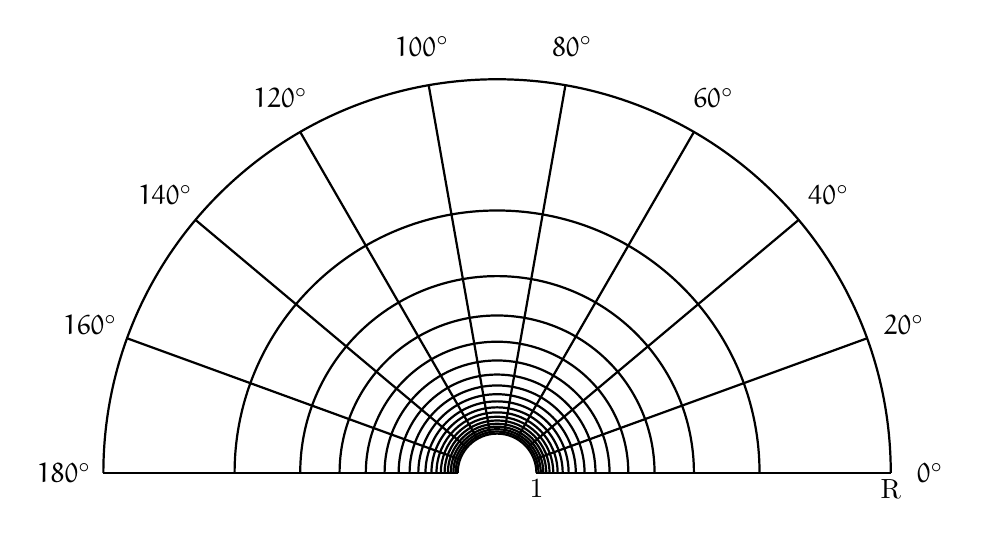
\begin{tikzpicture}
    			%Circles     
    			\foreach \r in {1, 1.05263, 1.11111, 1.17647, 1.25, 1.33333, 1.42857, 1.53846, 1.66667, 1.81818, 2, 2.22222, 2.5, 2.85714, 3.33333, 4, 5, 6.66667, 10}
      			\draw[thick] ({\r / 2},0) arc (0:180:{\r / 2});
    
    			%Rays
    			\foreach \a in {0, 20,...,180}
      			\draw[thick] (\a:.5) -- (\a:5);
   
     		\draw (.5,-.2) node {1};
     		\draw (5,-.2) node {R};
      
    			%Angle labels  
    			\foreach \a in {0, 20,...,180}
      			\draw (\a: 5.5) node {$\a^\circ$};
  		\end{tikzpicture}
  		\caption{Mesh around the body}
	\end{figure}		
	
	\begin{figure}
		\centering
  		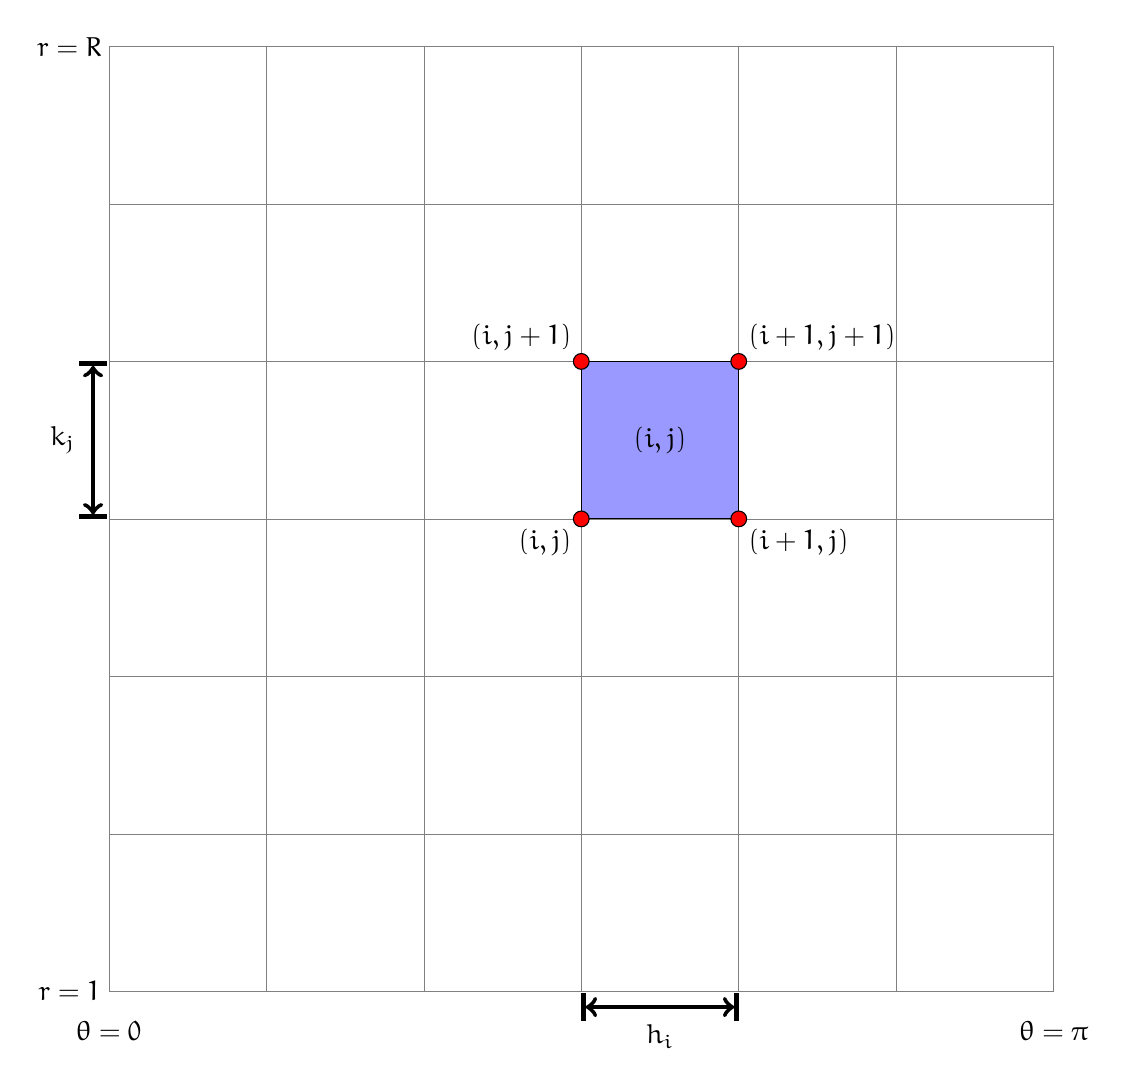
\begin{tikzpicture}
    			\draw[step=2,gray,very thin] (-6,-6) grid (6,6);
    			\filldraw[fill=blue!40!white, draw=black] (0,0) rectangle (2,2);
				\node[anchor=north east] (one) at (0,0) {$(i,j)$};
				\node[anchor=south east] (one) at (0,2) {$(i,j+1)$};
				\node[anchor=north west] (one) at (2,0) {$(i+1,j)$};
				\node[anchor=south west] (one) at (2,2) {$(i+1,j+1)$};
				\node (one) at (1,1) {$(i,j)$};

				\draw[fill=red] (0,0) circle(.1);
				\draw[fill=red] (2,0) circle(.1);
				\draw[fill=red] (0,2) circle(.1);
				\draw[fill=red] (2,2) circle(.1);

				\node (q) at (-6.5,-6) {$r=1$};
				\node (q) at (-6.5,6) {$r=R$};
				\node (q) at (-6,-6.5) {$\theta=0$};
				\node (q) at (6,-6.5) {$\theta=\pi$};

				\draw[|<->|, ultra thick] (0,-6.2) -- (2,-6.2);
				\node[anchor=north] (q) at (1,-6.3) {$h_i$};

				\draw[|<->|, ultra thick] (-6.2,0) -- (-6.2,2);
				\node[anchor=east] (q) at (-6.3,1) {$k_j$};
  		\end{tikzpicture}
  		\caption{Computational domain}
  		 \label{grid}
	\end{figure}	
	
	
	
	For a rectangular region $i,j$, $J[\chi]$ can be approximated as
	\begin{multline}
	J_{i,j} = p_\infty 
	\Biggl\{
		\Biggl[
			1 + \frac{(\gamma-1)M_\infty^2}{2T_{i,j}^2}
			\Biggl(
				T^2 - 1
				- 2\cos\theta '_i \frac{ \chi_{i,j+1} + \chi_{i+1,j+1} - \chi_{i,j} - \chi_{i+1,j}}{2k_j} \\
				+ \frac{2}{r'_j} \sin \theta '_i \frac{ \chi_{i+1,j} + \chi_{i+1,j+1} - \chi_{i,j} - \chi_{i,j+1}}{2h_i} \\
				- \left(
					\frac{ \chi_{i,j+1} + \chi_{i+1,j+1} - \chi_{i,j} - \chi_{i+1,j}}{2k_j}
				\right)^2 \\
				- \frac{1}{r^2}
				\left(
					\frac{ \chi_{i+1,j} + \chi_{i+1,j+1} - \chi_{i,j} - \chi_{i,j+1}}{2h_i}
				\right)^2
			\Biggr)
		\Biggr]^\alpha \\
		- 1 + \frac{\gamma M_\infty^2}{T_{i,j}^2}
		\Biggl(
			\left(
				\frac{r'^2_j-1}{r'^2_j}
			\right)
			\cos \theta '_i \frac{ \chi_{i,j+1} + \chi_{i+1,j+1} - \chi_{i,j} - \chi_{i+1,j}}{2k_j} \\
			- \left(
				\frac{r'^2_j-1}{r'^3_j}
			\right)
			\sin \theta '_i \frac{ \chi_{i+1,j} + \chi_{i+1,j+1} - \chi_{i,j} - \chi_{i,j+1}}{2h_i}
		\Biggr)
	 \Biggr\}
	\end{multline}
	$$	\theta '_i = \theta_i + 0.5h_i; \qquad r '_j = r_j + 0.5 k_j $$
	
	$$	
	T_{i,j}^2 = \frac{1}{r'^4_j}
	\left[
		(r'^2_j+\lambda^2)^2 - 4\lambda^2r'^2_j \cos^2 \theta '_i
	\right]	
	$$
	$$
	\lambda^2 = \frac{1-\tau}{1+\tau}
	$$
	Boundary conditions for $\chi$-
	\begin{enumerate}
	
	\item
	$$
	\frac{\partial \chi}{\partial r} = - \cos \theta; \text{ at } r=1
	$$
	\begin{equation}
	\chi_{i,1}=\frac{1}{k_2+2k_1}
	\left[
		\frac{1}{k_2}
		((k_1+k_2)^2\chi_{1,2} - k_1^2 \chi_{i,3})
		+ k_1(k_1+k_2)\cos \theta
	\right]
	\end{equation}
	
	\item $$ \frac{\partial \chi}{\partial \theta} = 0 \text{ at } \theta = 0, \pi $$
	\begin{equation}
	\chi_{m+1,j} = \chi_{m-1,j} \qquad 
	\chi_{0,j} = \chi_{2,j}
	\end{equation}
	
	\item $$ \chi = \frac{1}{R} \cos \theta \text{ as } r \rightarrow \infty $$
	\begin{equation}
	\chi_{i,n} = \frac{1}{R} \cos \theta_i
	\end{equation}
	
	\end{enumerate}
	
	Summing the contributions for each rectangle, $J[\chi]$ can be approximated as 
	\begin{equation}
	J[\chi] = \bar{J} = 
	\sum\limits_{i=1}^{n-1} \sum\limits_{j=1}^{m-1} J_{i,j}
	\end{equation}
	Therefore, the values of $\chi_{i,j}$ which maximizes this expression is given by the solutions of the equations
	\begin{equation}
	\frac{\partial \bar{J}}{\partial \chi_{i,j}} = 0
	\end{equation}
	$$ i = 1,\ldots,n $$
	$$ j = 2,\ldots,m-1 $$
	
	for a given $i,j$, the equation to maximize can be written in the form (by summing the contributions from the four surrounding rectangles)
	\begin{equation}
	\begin{split}
	g(\chi_{i,j}) = \frac{\partial \bar{J}}{\partial \chi_{i,j}} 
	\sum\limits_{s=(i,j),(i-1,j),(i,j-1),(i-1,j-1)}
	\Biggl[
		\alpha
		\left(
			A_s\chi^2_{i,j} + B_s\chi{i,j} + C_s
		\right)^{\alpha-1}
		\left(
			2A_s\chi_{i,j} + B_s
		\right) \\
		 + D_s
	\Biggr]H_s	
	= 0
	\end{split}
	\end{equation}
	
	Using Newton Raphson method, an improved estimate is given by
	\begin{equation}
	\chi^{(q+1)}_{i,j} = \chi^{(q)}_{i,j}
	- \frac{g(\chi^{(q)}_{i,j})}{g'(\chi^{(q)}_{i,j})}
	\end{equation}
	
	\begin{equation}
	g' = \frac{\partial g_{i,j}}{\partial \chi_{i,j}}
	\end{equation}
	
	
	\subsection{Coefficients A, B, C, D, H}
	The coefficients A, B, C, D, H are given by - 
	
	\begin{align}
		\begin{split}		
		A_{i,j} = -\frac{(\gamma-1)M_\infty^2}{2T_{i,j}^2}
		\left(
			\frac{1}{4k_j^2} + \frac{1}{4{r'}_j^2 h_i}
		\right) \\
		A_{i,j-1} = -\frac{(\gamma-1)M_\infty^2}{2T_{1,j-1}^2}
		\left(
			\frac{1}{4k_{j-1}^2} + \frac{1}{4{r'}_{j-1}^2 h_i}
		\right) \\
		A_{i-1,j} = -\frac{(\gamma-1)M_\infty^2}{2T_{i-1,j}^2}
		\left(
			\frac{1}{4k_j^2} + \frac{1}{4{r'}_j^2 h_{i-1}}
		\right) \\
		A_{i-1,j-1} = -\frac{(\gamma-1)M_\infty^2}{2T_{i-1,j-1}^2}
		\left(
			\frac{1}{4k_{j-1}^2} + \frac{1}{4{r'}_{j-1}^2 h_{i-1}}
		\right)
		\end{split}
	\end{align}
	
	\begin{equation}
		\begin{split}
		B_{i,j} = \frac{(\gamma-1)M_\infty^2}{2T_{i,j}^2}
		\Biggl(
			2\cos \theta '_i \frac{1}{2k_j}
			- \frac{2}{r'_j} \sin\theta '_i \frac{1}{2h_i} \\
			+ \frac{1}{2k_j^2}( \chi_{i,j+1} + \chi_{i+1,j+1} - \chi_{i+1,j} ) \\
			+ \frac{1}{2r'^2_jh_i^2}( \chi_{i+1,j} + \chi_{i+1,j+1} - \chi_{i,j+1} )
		\Biggr) \\
		B_{i,j-1} = \frac{(\gamma-1)M_\infty^2}{2T_{i,j-1}^2}
		\Biggl(
			- 2\cos \theta '_i \frac{1}{2k_{j-1}}
			- \frac{2}{r'_{j-1}} \sin\theta '_i \frac{1}{2h_i} \\
			- \frac{1}{2k_{j-1}^2}( \chi_{i+1,j} - \chi_{i,j-1} - \chi_{i+1,j-1} ) \\
			+ \frac{1}{2r'^2_{j-1}h_i^2}( \chi_{i+1,j-1} + \chi_{i+1,j} - \chi_{i,j-1} )
		\Biggr) \\
		B_{i-1,j} = \frac{(\gamma-1)M_\infty^2}{2T_{i-1,j}^2}
		\Biggl(
			2\cos \theta '_{i-1} \frac{1}{2k_j}
			+ \frac{2}{r'_j} \sin\theta '_{i-1} \frac{1}{2h_{i-1}} \\
			+ \frac{1}{2k_j^2}( \chi_{i-1,j+1} + \chi_{i,j+1} - \chi_{i-1,j} ) \\
			- \frac{1}{2r'^2_jh_{i-1}^2}( \chi_{i,j+1} - \chi_{i-1,j+1} - \chi_{i-1,j+1} )
		\Biggr) \\
		B_{i-1,j-1} = \frac{(\gamma-1)M_\infty^2}{2T_{i-1,j-1}^2}
		\Biggl(
			- 2\cos \theta '_{i-1} \frac{1}{2k_{j-1}}
			+ \frac{2}{r'_{j-1}} \sin\theta '_{i-1} \frac{1}{2h_{i-1}} \\
			- \frac{1}{2k_{j-1}^2}( \chi_{i-1,j} - \chi_{i-1,j-1} - \chi_{i,j-1} ) \\
			- \frac{1}{2r'^2_{j-1}h_{i-1}^2}( \chi_{i,j-1} - \chi_{i-1,j-1} - \chi_{i-1,j} )
		\Biggr) \\
		\end{split}
	\end{equation}
	
	\begin{equation}
		\begin{split}
		C_{i,j} = 1 + \frac{(\gamma-1)M_\infty^2}{2T_{i,j}^2}
		\Biggl(
			T_{i,j}^2 - 1
			- \frac{\cos \theta '_i}{k_j}( \chi_{i,j+1} + \chi_{i+1,j+1} - \chi_{i+1,j} ) \\
			+ \frac{\sin \theta '_i}{r'_j h_i}( \chi_{i+1,j} + \chi_{i+1,j+1} - \chi_{i,j+1} ) \\
			- \frac{1}{4k_j^2}( \chi_{i,j+1} + \chi_{i+1,j+1} - \chi_{i+1,j} )^2 \\
			- \frac{1}{4r'^2_j h_i^2}( \chi_{i+1,j} + \chi_{i+1,j+1} - \chi_{i,j+1} )^2
		\Biggr) \\
		C_{i,j-1} = 1 + \frac{(\gamma-1)M_\infty^2}{2T_{i,j-1}^2}
		\Biggl(
			T_{i,j-1}^2 - 1
			- \frac{\cos \theta '_i}{k_{j-1}}( \chi_{i+1,j} - \chi_{i,j-1} - \chi_{i+1,j-1} ) \\
			+ \frac{\sin \theta '_i}{r'_{j-1} h_i}( \chi_{i+1,j-1} + \chi_{i+1,j} - \chi_{i,j-1} ) \\
			- \frac{1}{4k_{j-1}^2}( \chi_{i+1,j} - \chi_{i,j-1} - \chi_{i+1,j-1} )^2 \\
			- \frac{1}{4r'^2_{j-1} h_i^2}( \chi_{i+1,j-1} + \chi_{i+1,j} - \chi_{i,j-1} )^2
		\Biggr) \\
		C_{i-1,j} = 1 + \frac{(\gamma-1)M_\infty^2}{2T_{i-1,j}^2}
		\Biggl(
			T_{i-1,j}^2 - 1
			- \frac{\cos \theta '_{i-1}}{k_j}( \chi_{i-1,j+1} + \chi_{i,j+1} - \chi_{i-1,j} ) \\
			+ \frac{\sin \theta '_{i-1}}{r'_j h_i}( \chi_{i,j+1} - \chi_{i-1,j+1} - \chi_{i-1,j+1} ) \\
			- \frac{1}{4k_j^2}( \chi_{i-1,j+1} + \chi_{i,j+1} - \chi_{i-1,j} )^2 \\
			- \frac{1}{4r'^2_j h_{i-1}^2}( \chi_{i,j+1} - \chi_{i-1,j+1} - \chi_{i-1,j+1} )^2
		\Biggr) \\
		C_{i-1,j-1} = 1 + \frac{(\gamma-1)M_\infty^2}{2T_{i-1,j-1}^2}
		\Biggl(
			T_{i-1,j-1}^2 - 1
			- \frac{\cos \theta '_{i-1}}{k_{j-1}}( \chi_{i-1,j} - \chi_{i-1,j-1} - \chi_{i,j-1} ) \\
			+ \frac{\sin \theta '_{i-1}}{r'_{j-1} h_{i-1}}( \chi_{i,j-1} - \chi_{i-1,j-1} - \chi_{i-1,j} ) \\
			- \frac{1}{4k_{j-1}^2}( \chi_{i-1,j} - \chi_{i-1,j-1} - \chi_{i,j-1} )^2 \\
			- \frac{1}{4r'^2_{j-1} h_{i-1}^2}( \chi_{i,j-1} - \chi_{i-1,j-1} - \chi_{i-1,j} )^2
		\Biggr) \\
		\end{split}
	\end{equation}
	
	\begin{equation}
		\begin{split}
		D_{i,j} = -1 + \frac{\gamma M_\infty^2}{T_{i,j}^2}
		\Biggl[
			-
			\left(
				\frac{r'^2_j - 1}{r'^2_j}
			\right)
			 \frac{\cos \theta '_i}{2k_j}
			+ 			
			\left(
				\frac{r'^2_j - 1}{r'^3_j}
			\right)
			 \frac{\sin \theta '_i}{2h_i}
		\Biggr] \\
		D_{i,j-1} = -1 + \frac{\gamma M_\infty^2}{T_{i,j-1}^2}
		\Biggl[
			\left(
				\frac{r'^2_{j-1} - 1}{r'^2_{j-1}}
			\right)
			 \frac{\cos \theta '_i}{2k_{j-1}}
			+ 			
			\left(
				\frac{r'^2_{j-1} - 1}{r'^3_{j-1}}
			\right)
			 \frac{\sin \theta '_i}{2h_i}
		\Biggr] \\
		D_{i-1,j} = -1 + \frac{\gamma M_\infty^2}{T_{i-1,j}^2}
		\Biggl[
			- 
			\left(
				\frac{r'^2_j - 1}{r'^2_j}
			\right)
			 \frac{\cos \theta '_{i-1}}{2k_j}
			- 			
			\left(
				\frac{r'^2_j - 1}{r'^3_j}
			\right)
			 \frac{\sin \theta '_{i-1}}{2h_{i-1}}
		\Biggr] \\
		D_{i-1,j-1} = -1 + \frac{\gamma M_\infty^2}{T_{i-1,j-1}^2}
		\Biggl[
			\left(
				\frac{r'^2_{j-1} - 1}{r'^2_{j-1}}
			\right)
			 \frac{\cos \theta '_{i-1}}{2k_{j-1}}
			-		
			\left(
				\frac{r'^2_{j-1} - 1}{r'^3_{j-1}}
			\right)
			 \frac{\sin \theta '_{i-1}}{2h_{i-1}}
		\Biggr] \\
		\end{split}
	\end{equation}
	
	\begin{equation}
		\begin{split}
			H_{i,j} = r'_j T_{i,j}^2 h_i k_j \\
			H_{i,j-1} = r'_{j-1} T_{i,j-1}^2 h_i k_{j-1} \\
			H_{i-1,j} = r'_j T_{i-1,j}^2 h_{i-1} k_j \\
			H_{i-1,j-1} = r'_{j-1} T_{i-1,j-1}^2 h_{i-1} k_{j-1} 
		\end{split}
	\end{equation}
	
	\chapter{Conclusion}
	\section{Summary}
	
	
	
\begin{thebibliography}{9}	

	\bibitem{rasmussen}
  		H. Rasmussen, and N. Heys,
  		\emph{Application of a Variational Method in Plane Compressible Flow Calculation},
  		Aeronautical Research Council Current Papers
  		1974.

	\bibitem{multigrid}
  		William L. Briggs, Van Emden Henson, and Steve F. McCormick,
  		\emph{A Multigrid Tutorial},
  		SIAM
  		2nd Edition
  		2000.
  		
	\bibitem{cuda}
  		NVIDIA CUDA Zone,
  		\emph{https://developer.nvidia.com/how-to-cuda-c-cpp}
  		
	\bibitem{mapreduce}
  		James Gain, Michelle Kuttel, Sebastian Wyngaard,
Simon Perkins and Jason Brownbridge,
		\emph{Parallel Algorithms},
  		\emph{http://people.cs.uct.ac.za/~jgain/lectures/Algorithms.pdf}



\end{thebibliography}

\end{document}
